% !TEX root = ../notes_template.tex
\chapter{Hierarchical Models and Laplace Approximation}\label{chp:hierarchical_models}

\section{Why Hierarchical Models are Necessary} \label{sec:Chap2_why}

In Chapter 1, we saw that most ecological processses can be represented as an individual-based model (IBM), and that often we can approximate these IBMs using a statistical model fitted using maximum likelihood. We also saw that maximum likelihood estimation involves specifying a model that results in a probability distribution for data given some set of parameters \( \theta \), and then maximizing this log-likelihood with respect to parameters to get the estimator \( \hat{\theta} \).  However, there are at least three different reasons to extend maximum likelihood estimation to include some variables that are marginalized across (called \myindex{random effects}).  

\begin{enumerate}
    \item \textit{Distribution for data has no simple expression}: In many cases, we cannot write a probability density for data directly as a function of parameters.  For example, in Jolly-Seber capture-recapture models \cite{jolly_explicit_1965,seber_note_1965}, we observe a sequence of times when a tagged organism is encountered, and want to infer birth and death times while estimating survival and detection probabilities. It is not immediately clear how to write out the probability density for when the animal was encountered given survival and detection probabilities.  However, it is possible to write down this probability when introducing additional latent (unobserved) processes (i.e., the latent time of birth and death for each animal), and then defining the data conditional upon these;

    \item \textit{Data are not independent}:  As we saw, it is often convenient to write the full log-likelihood by calculating the log-likelihood for each datum individually and then summing across these.  However, these two are equivalent only when residuals are independent for each sample.  In the following, we are concerned with situations when residuals are correlated across space or time, and these correlated residuals will make it impossible to calculate the log-likelihood of data by simply summing the log-likelihood of each datum individually.  For example, ecologists are trained to avoid \textit{pseudoreplication} that arises when experimental replicates are not independent, e.g., because experimental sites are located near one-another and hence have similar ecological characteristics that are not under experimental control \cite{hurlbert_pseudoreplication_1984}.  However, we might still gain useful information while analyzing data from a pseudoreplicated design by modelling correlations that result from these uncontrolled factors;

    \item \textit{Improved performance using shrinkage estimators}: Statisticians described the Stein paradox decades ago \cite{stein_inadmissibility_1956}, wherein an analyst can average measurements for different things (termed ``sampling units") to decrease the expected error for each.  This method is paradoxical because it could involve averaging measurements for sampling units that are completely unrelated, like batting averages for baseball players and the proportion of rainy days in different cities.  Statisticians later resolved this paradox by defining the concept of \myindex{shrinkage}, where we estimate the variance in some measurement among sampling units, and the ratio of measurement and among-unit variance defines how much we ``shrink" estimates towards one-another \cite{efron_steins_1977}.  Random effects introduce a general method for defining \textit{shrinkage estimators} that can often improve statistical efficiency.  
\end{enumerate}
There is a large vocabulary of different ways of describing models that include random effects, including \textit{hierarchical models}, \textit{mixed-effect models}, \textit{multi-level models}, \textit{data augmentation}, \textit{empirical Bayes}, and many others.  These different vocabularies arise from different ways that random effects can be derived, and have subtle differences in how models are interpreted.  However, these differences are not relevant in the following, so we will proceed by referring to \myindex{mixed-effects models} as those that have both random and fixed effects. 

Before we continue further, however, we will illustrate the first reason using a common ecological example, wherein an analyst samples the total biomass in a given area.  This arises frequently in fisheries surveys \cite{maureaud_are_2021}, but also for insect light traps \cite{zhou_long-term_2023}, plant pollen traps \cite{giesecke_early_2010}, and other settings.  

\subsection{Example: Compound distributions} \label{sec:Chap2_compound_distribution}

In Section \ref{sec:Chap1_point_process}, we introduced a Poisson point process, where organisms are located randomly and independently such that the number of individuals in a specified area follows a Poisson distribution\footnote{See https://github.com/james-thorson/Spatio-temporal-models-for-ecologists/Chap\_2 for code associated with this chapter.}.  However, ecologists often study not just the density of individuals but also their sizes.  To explore this, we might assume that individuals have two marks, representing location \(S_i\) and size measured as organism biomass \(W_i\).  We specifically seek to identify a distribution for the total biomass \(B\) in a given area \(A\), \( B = \sum_{i=1}^{N} W_i \). 

To envision this process, we specify a distribution for the number of animals \(N\) in a defined area and the size of each such animal \(W_i\).  For simplicity, we will assume that animals are distributed independently, such that abundance \(N\) follows a Poisson distribution, and that organism sizes follow a Gamma distribution:

\begin{equation} \label{eq:Chap2_CPG}
\begin{gathered}
    N \sim \mathrm{Poisson}( \lambda_A ) \\
    W_i \sim \mathrm{Gamma}( k, \theta )  
\end{gathered}
\end{equation}
where \( \lambda_A = \int_{s \in A} \lambda(s) ds \) and \(\lambda(s)\) is the expected density of individuals at any location \(s\).  

The resulting distribution for \( B \) is called a \myindex{compound probability distribution}.  It is straightforward to simulate from this distribution by:
\begin{enumerate}
  \item simulating the number of organisms \(N\) from a Poisson distribution;
  \item for each organism, simulate it's biomass from a Gamma distribution;
  \item add together the biomass from each organism
\end{enumerate}
where these steps correspond to the components in Eq. \ref{eq:Chap2_CPG}.  This corresponds to taking a draw from the probability distribution from the compound distribution, which we call a Poisson-gamma distribution because it is formed from these two component processes. We can therefore simulate from this compound distribution, even though we can't write down the probability distribution \( f(B | \lambda_A, k, \theta ) \) in a simple expression.  Unfortunately, we need this probability distribution to then calculate the likelihood and use this to estimate parameters.  

To calculate this probability density (or the density of any other compound distribution), we could first try calculating the density given a hypothetical value for \(N\), corresponding to some perfect knowledge about how many organisms are present in that area:

\begin{equation}
\begin{aligned}
    f_{N=0}( B | N = 0, k, \theta ) &= 
    \begin{cases}
        1 & \text{if } B=0 \\ 
        0 & \text{if } B>1 
    \end{cases} \\
    f_{N=1}( B | N = 1, k, \theta ) &= \mathrm{dGamma}( B | k, \theta ) \\
    f_{N=2}( B | N = 2, k, \theta ) &= \mathrm{dGamma}( B | 2k, \theta ) \\
    ... \\
    f_{N=n}( B | N = n, k, \theta ) &= \mathrm{dGamma}( B | nk, \theta )
%\end{gathered}
\end{aligned}
\end{equation}
where \(\mathrm{dGamma}(B | k,\theta)\) evaluates a gamma probability density function for response \(B\) given shape \(k\) and scale \(\theta\).  We additionally know the probability that \( N = n \) individuals are present follows a Poisson distribution. Writing this more succinctly, we see:

\begin{equation} \label{eq:Chap2_Compound_Poisson_Gamma}
    f( B | \lambda_A, k, \theta ) = \sum_{N=0}^{\infty} \mathrm{dGamma}( B | Nk, \theta ) \mathrm{dPoisson}(N|\lambda_A) 
\end{equation}
where \(\mathrm{dPoisson}\) evaluates the Poisson probability mass function.  We will use specialized terms for the different components of this expression.  We call:
\begin{itemize}
    \item \( N \) a \myindex{latent variable}, because it affects the likelihood of our data \(B\) without itself being directly observable;

    \item \(\mathrm{dPoisson}(N|\lambda_A)\) the marginal distribution for the latent variable;

    \item \(\mathrm{dGamma}( B | Nk, \theta )\) the conditional distribution for the data given a value of the latent variable;
    
    \item \( \mathrm{dGamma}( B | nk, \theta ) \mathrm{dPoisson}(n|\lambda_A) \) the ``joint distribution" because it includes the distribution of both our observable data \(B\) and our unobservable random effect;

    \item \( f( B | \lambda_A, k, \theta ) \) the marginal distribution for the data because it is calculated by \myindex{marginalizing} across the latent variable, \(N\).  
\end{itemize}
This example therefore takes the marginal distribution for a latent variable, the conditional distribution for the data given this latent variable, and uses these to calculate the marginal distribution for the data.  We can later do the same process in reverse to calculate the likelihood of parameters \(k\), \(\theta\), and \(\lambda\).  

This compound Poisson-gamma distribution arises often in ecological studies, and statisticians have developed efficient techniques to evaluate it as a Tweedie distribution \cite{foster_poissongamma_2013}:

\begin{equation}
    W_A \sim \mathrm{Tweedie}( \mu_A, \phi_A, p )
\end{equation}
where \( \mu_A = \lambda_A k \theta \), \( \phi_A = \theta(k+1)\mu_A^\frac{-1}{k+1} \), and \( p = \frac{k+2}{k+1} \) \cite{thorson_diet_2022}.  
Importantly, the Tweedie distribution includes a non-zero probability of observing mass \(B=0\), and this arises when the Poisson distribution yields a count of zero animals.  However, the compound Poisson-gamma distribution then also admits continuous values for total mass \(B>0\).  

Other compound distributions that arise often for ecologists include:
\begin{itemize}
    \item \textit{Negative binomial distribution}\index{negative binomial distribution}:  the negative binomial arises as a Poisson distribution, where the Poisson intensity \(\lambda^*\) itself follows a Gamma distribution.  
    
\begin{equation} \label{eq:Chap2_Negative-Binomial}
\begin{gathered}
    \lambda^* \sim \mathrm{Gamma}(k, \theta) \\
    N \sim \mathrm{Poisson}(\lambda^*)
\end{gathered}
\end{equation}
    where shape \(k = \frac{1}{\sigma^2}\) and scale \( \theta = \lambda \sigma^2 \), and \( \sigma \) is the coefficient of variation for the Gamma distribution while \(\lambda\) is again the average density of individuals.  This compound distribution is useful to represent a point process where animals are clustered in space or time, where the gamma distribution represents fine-scale variation in density \cite{linden_using_2011};

    \item \textit{{Lognormal-Poisson distribution}}\index{lognormal-Poisson distribution}:  as an alternative to the negative binomial, we could instead assume that spatial clustering arises from a lognormal process:
    
\begin{equation} \label{eq:Chap2_Lognormal-Poisson}
\begin{gathered}
    \log(\lambda^*) \sim \mathrm{Normal}( \mu, \sigma^2) \\
    N \sim \mathrm{Poisson}(\lambda^*)
\end{gathered}
\end{equation}
    where \( \sigma \) is the log-standard deviation of overdispersion, and \(\mu\) is the log-density.  Although the  lognormal-Poisson distribution is less widely used than the negative binomial, normally distributed variation in the log-intensity is the simplest form of what's called a \myindex{log-Gaussian Cox process};  
    
    \item \myindex{Dirichlet-multinomial distribution}: in a point process involving \(C\) categorical marks (i.e., taxa, sizes, ages, etc.), the multinomial distribution is useful to represent the count \(N_c\) for each category \(c \in \{1,2,...,C\}\) given a known total count \( n = \sum_{c=1}^{C} N_c \) across categories.  The Dirichlet-multinomial distribution then generalizes this by approximating a Poisson point process where each species is spatially clustered \cite{thorson_model-based_2016}. For example, we might specify an average proportion \(\mathbf{p}\) for each category, but where a given site has proportion \(\mathbf{p}^*\) that differs due to small-scale variation in habitat:

\begin{equation} \label{eq:Chap2_Dirichlet-multinomial}
\begin{gathered}
    \mathbf{p}^* \sim \mathrm{Dirichlet}( \alpha \mathbf{p} ) \\ 
    \mathbf{N} \sim \mathrm{Multinomial}( \mathbf{p}^*, n ) 
\end{gathered}
\end{equation}
    where the variance of the Dirichlet distribution decreases as \( \alpha \) increases, such that the compound Dirichlet-multinomial distribution reverts to a standard multinomial distribution as \( \alpha \rightarrow \infty \).  
    
\end{itemize}

In each of these compound distributions, the marginal distribution is then obtained by marginalizing across the outcome of some underlying latent variable.  However, it is helpful to be familiar with these distributions because:

\begin{enumerate}
    \item \textit{Closed-form calculation}: the negative binomial and Dirichlet-multinomial distributions also have a closed form expression for evaluating the likelihood, and therefore can be fitted with little computational cost;
    
    \item \textit{Computational efficiency}: the Tweedie distribution is implemented in many packages, using several computational tricks to promote computational efficiency;
    
    \item \textit{Simplified explanation}: each of these distributions is commonly encountered across ecological models, and therefore can be described without needing extensive background for readers.  
\end{enumerate}

\subsection{A Quick Derivation of Random Effects} \label{sec:Chap2_deriving_random_effects}

We next seek to generalize the process that was presented in Section \ref{sec:Chap2_compound_distribution} when calculating the compound Poisson-gamma distribution, so that we can use it during maximum likelihood estimation.  To do so, we first introduce two concepts:

\begin{itemize}
    \item \textit{Axiom of total probability}\index{axiom of total probability}:  say we have two events \(X\) and \(Y\).  We can re-write a joint probability distribution \(\Pr(X,Y)\) as the product of a conditional and marginal distribution:
\begin{equation}
    \Pr(X,Y) = \Pr(Y|X) \Pr(X)
\end{equation}
    This is how we've formulated each compound distribution (e.g., \ref{eq:Chap2_Dirichlet-multinomial}, \ref{eq:Chap2_Lognormal-Poisson}, and \ref{eq:Chap2_Negative-Binomial}), where it is easier to specify a conditional probability \( \Pr(Y|X) \) and the marginal probability of a latent variable \( \Pr(X) \) than specify the joint probability \( \Pr(X,Y) \);
    
    \item \textit{Law of total probability}\index{law of total probability}:  similarly, we can marginalize a joint probability to get a marginal probability.  If the latent variable \(X\) is continuous-valued, this involves an integral:
\begin{equation}
    \Pr(Y) = \int \Pr(X,Y) \mathrm{d} X    
\end{equation}
    Alternatively, if latent variable \(X\) is discrete-valued with values \( \Omega \), this involves a summation as we already saw in Eq. \ref{eq:Chap2_Compound_Poisson_Gamma}:
\begin{equation}
    \Pr(Y) = \sum_{x \in \Omega} \Pr(Y,X=x)    
\end{equation}
    In either case, it tends to require some careful thought to find a computationally efficient way to marginalize across latent variable \(X\).  

\end{itemize}
In essence, the axiom of total probability allows us to construct a joint probability from a marginal and conditional probability, while the law of total probability allows us to recover a marginal from a joint probability.  

Next, we introduce a vector of latent variables \( \mathbf{\epsilon} \), where we can define a distribution for data given these variables, \( \Pr(Y | \theta, \mathbf{\epsilon}) \), and can also specify a distribution for them \( \Pr( \mathbf{\epsilon} | \theta) \).  By the Axiom of Total Probability, the product of these two is the joint probability of data and random effects.  Then, by the Law of Total Probability, we can integrate this to get the marginal likelihood of parameters:

\begin{equation}
    \mathcal{L}( \theta; Y ) = \int \Pr(Y | \theta, \mathbf{\epsilon}) \Pr( \mathbf{\epsilon} | \theta) \mathrm{d} \mathbf{\epsilon}
\end{equation}
This derivation shows that we can still calculate \( \hat{\theta} \) by maximizing \( \log \mathcal{L}( \theta; y ) \), but in some cases it requires introducing random effects \(\mathbf{\epsilon}\) which we then marginalize across (either using summation or integration).  

After identifying \( \hat{\theta} \), we also define the ``empirical Bayes" predictions for random effects:
\begin{equation} \label{eq:Chap2_empirical_bayes}
    \hat{\mathbf{\epsilon}} = \mathrm{argmax}_{\mathbf{\epsilon}} \Pr(Y | \hat{\theta}, \mathbf{\epsilon}) \Pr( \mathbf{\epsilon} | \hat{\theta})
\end{equation}
These empirical Bayes predictions \( \hat{\mathbf{\epsilon}} \) are affected both by data \( \Pr(Y | \hat{\theta}, \mathbf{\epsilon}) \) but are also shrunk towards a distribution \( \Pr( \mathbf{\epsilon} | \hat{\theta}) \) that is affected by estimated parameters \(\hat{\theta}\), such that the empirical Bayes estimator generalizes the properties of James-Stein shrinkage. However, calculating \( \mathcal{L}( \theta; Y ) \) requires an integral across \( \mathbf{\epsilon} \), which we call ``random effects". 

\section{Introducing the Laplace Approximation} \label{sec:Chap2_Laplace}

We next introduce the \myindex{Laplace approximation}, which can be a computationally efficient way of computing the integral (called \textit{integration}) across random effects.  Ecologists generally receive some background in integration and may recall that it can be conducted analytically by identifying an antiderivative for a given function.  However, analytical integration is generally harder than analytical differentiation, and we again suspect that most ecologists are unlikely to investigate a function by integrating it analytically.  We therefore introduce several techniques to compute an integral (Table \ref{tab:Chap2_integration}) but generally emphasize the Laplace approximation due to its computationally efficiency when combined with automatic differentiation (Table \ref{tab:Chap1_differentiation}) \cite{skaug_automatic_2006}.

\begin{table}
  \caption[Methods used for integration]{List of methods used throughout the textbook to calculate the area or volume under a function (called \myindex{integration}), where these methods provide an inverse for differentiation (Table \ref{tab:Chap1_differentiation}).}
\begin{center}
\begin{tabularx}{\textwidth}{ | X m{3.5in} | } 
  \hline
  Name & Description \\ 
  \hline

  Analytical & Memorizing many well-known transformations and applying them in clever ways (e.g., using u-substitution) to function \( f(x) \) to define the antiderivative \( F(x) \) that can later be evaluated to calculate a definite or indefinite integral given some bounds \\ & \\ 
  
  Monte Carlo & Evaluating function \( f(x) \) at some randomized set of points, and computing the integral via the evaluated values at those randomized points \\ & \\

  Rejection sampling & Randomly sampling points \(x\) from the domain of \(f(x)\) and either rejecting or accepting them, where the accepted points then approximates the target function \(f(x)\) and can be used to integrate some transformation of that function (Section \ref{sec:rejection_sampling}) \\ & \\

  Markov chain Monte Carlo (MCMC) sampling & Randomly sampling a sequence of points \(x\) and either accepting or rejecting changes that occur during that sequence, such that the sequence of values then approximate the target function \(f(x)\), with use similar to rejection sampling \\ & \\

  Laplace approximation & Approximating the joint likelihood \(f(x)\) as if it follows a normal distribution with the same peak value, location, and curvature (see Section \ref{sec:Chap2_Laplace}) \\
  
  \hline
\end{tabularx}
  \label{tab:Chap2_integration}
\end{center}
\end{table}

At it's core, the Laplace approximation replaces any integral with a multivariate normal distribution that has similar properties, and calculates the area under that multivariate normal distribution \cite{skaug_automatic_2006}.  To approximate the integral for a function \(g(\theta)\) it requires calculating:
\begin{enumerate}
    \item \textit{Location of peak}: the value \(\hat{\theta}=\mathrm{argmax}_{\theta} (\log(g(\theta)))\) that maximizes the function;

    \item \textit{Value at peak}: the function value \( \log(g(\hat{\theta})) \) at this peak;

    \item \textit{Curvature at peak}: the curvature of the function at this peak, measured as the second derivative of \(\log(g)\) around \(\hat{\theta}\), \( h = \frac{\mathrm{d}^2}{\mathrm{d}\theta^2} \log(g(\hat{\theta}))\). 
\end{enumerate}
The Laplace approximation then substitutes \(g\) with a normal distribution having those same three values.  The normal distribution has density:

\begin{equation}
    \mathrm{dNormal}( x | \mu, \sigma ) = \frac{1}{\sigma \sqrt{2 \pi}} e^{ -0.5(x-\mu)^2\sigma^{-2} }
\end{equation}
where \( \sigma \) is the standard deviation and \( \mu \) is the mean of the distribution, and (like any probability) the area under this distribution is equal to 1.  Therefore, if a distribution \(g\) has the same shape as the normal distribution, but has peak with value \(g(\hat{x})\) and \(\log(g)\) has curvature \(h\), then the integral for \(g\) will be approximately:

\begin{equation} \label{eq:Chap2_univariate_Laplace}
    \log \left(\int g(\theta) \mathrm{d}\theta \right) \approx \sqrt{2\pi} \log \left( g(\hat{\theta}) \right) 0.5h
\end{equation}

Similarly, the Laplace approximation can be applied to approximate a function \(g(\mathbf{\theta})\) where \(\mathbf{\theta}\) has two or more dimensions.  In this case, we approximate the function using a multivariate normal distribution, which has density:

\begin{equation} \label{eq:Chap2_MVN}
    \mathrm{dMVN}(\mathbf{x}|\mathbf{\mu,\Sigma}) = \frac{\sqrt{|\mathbf{Q}|}}{(2\pi)^{k/2}} e^{-0.5\mathbf{(x-\mu)}^T \mathbf{Q (x-\mu)}}
\end{equation}
where \(\mathbf{Q} = \mathbf{\Sigma}^{-1}\) is the inverse of the covariance matrix and \(|\mathbf{Q}|\) is the determinant of this matrix.  \(\mathbf{Q}\) will come up often in subsequent chapters, and is often specifically called the \myindex{precision matrix}.  Importantly, the precision matrix \(\mathbf{Q}\) and not the covariance matrix \(\mathbf{\Sigma}\) appears in the multivariate normal distribution, so we will often look for ways to compute the precision matrix \(\mathbf{Q}\), rather than constructing the covariance matrix \(\mathbf{\Sigma}\) and then inverting it (because this matrix inverse step is computationally expensive).  As we saw in Section \ref{sec:Chap1_likelihood_GLM}, we can measure the curvature using precision \(\mathbf{Q}\) by calculating a matrix of second derivatives of \(\log(g)\), called the Hessian matrix \(\mathbf{H}\).   

Extending Eq. \ref{eq:Chap2_univariate_Laplace}, if a function has peak with value \(g(\hat{\theta})\) with \(\log(g)\) has curvature \(\mathbf{H}\), we can approximate the integral using a multivariate normal distribution with those same characteristics:

\begin{equation} \label{eq:Chap2_multivariate_Laplace}
    \log \left( \int g(\theta) \mathrm{d}\theta \right) \approx (2\pi)^{k/2} \log \left( g(\hat{\theta}) \right) 0.5 |\mathbf{H}|
\end{equation}
where \(|\mathbf{H}|\) is the determinant of this Hessian matrix.  This then reverts to Eq. \ref{eq:Chap2_univariate_Laplace} when \(g\) has only a single dimension but generalizes it for two or more dimensions, and we present both because the univariate version might be more familiar to some readers.

We first show how the Laplace approximation is used to approximate a univariate integral (Eq. \ref{eq:Chap2_univariate_Laplace}) using a simple example with a known ``Chi-squared" distribution, so we can compare the Laplace approximation with the true value.  The chi-squared distribution has a known density function:

\begin{equation}
    \Pr(X=x | k) = \frac{1}{2^{k/2} \Gamma(k/2)} x^{k/2-1}e^{-x/2}\
\end{equation}
Taking the log and eliminating the component that does not depend on \(x\):

\begin{equation}
    \log \left(\Pr(X=x | k) \right) \propto f(x|k) \\
                            = \left(\frac{k}{2}-1\right) \log(x) - \frac{x}{2}
\end{equation}
We then calculate the first derivative:

\begin{equation} \label{eq:Chap2_Chi2_derivative}
    f'(x|k) = \left(\frac{k}{2}-1\right)x^{-1} - \frac{1}{2}
\end{equation}
The peak of this function then occurs where  \( f'(x|k)=0 \), and solving Eq. \ref{eq:Chap2_Chi2_derivative} for \(x\) shows that this occurs when \(\hat{x}=k-2\).  Substituting this into Eq. \ref{eq:Chap2_Chi2_derivative} and then taking the second derivative yields:

\begin{equation}
    f''(\hat{x}|k) = \frac{1}{2(k-2)}
\end{equation}
We can therefore approximate the chi-squared distribution with a normal distribution that has the same peak and a variance equal to \( 1/f''(\hat{x}|k) \):

\begin{equation}
    \log \left( \Pr(X=x | k) \right) \propto \log \left( \mathrm{dNormal}( x | \mu=k-2, \sigma^2=2(k-2) ) \right)
\end{equation}

Alternatively, we can do this without calculating derivatives algebraically, and instead use the function \colorbox{backcolour}{D} in R to do ``symbolic differentiation" (see Code \ref{code:Chap2-R-Laplace-approximation}).  We used symbolic differentiation previously in Section \ref{sec:Chap1_time_to_event} to simplify calculating the distribution for age-at-death, and here show that the same can be done when calculating the Laplace approximation.  As this code demonstrates, the area under this normal approximation can be calculated as:

\lstset{style=Rcode}
\lstinputlisting[language=R, label=code:Chap2-R-Laplace-approximation, firstline=18, lastline=47, caption=R code visualizing Laplace approximation for the chi-squared distribution using symbolic differentiation., captionpos=t]{Chap_2/Laplace_examples.R}

\begin{figure}[!ht]
    \caption[Laplace example using chi-squared distribution]{A chi-square distribution with \(k={5, 25, 100}\) degrees of freedom (black lines) and the normal approximation (blue lines) that has the same mode, peak, and curvature (2nd derivative evaluated at the peak), and listing the area under the curve for the normal approximation calculated using the Laplace method (blue legend).}
    \centering
    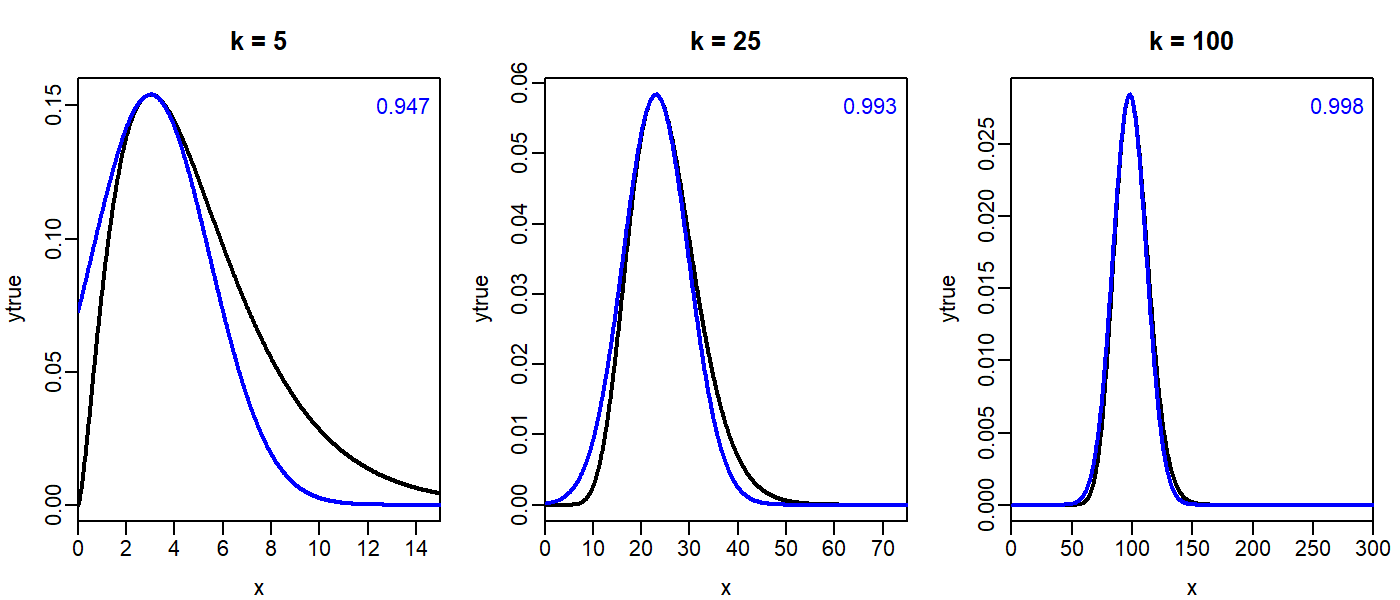
\includegraphics[width=5.5in]{Chap_2/Laplace_demo.png}
    \label{fig:Chap2_laplace}
\end{figure}

\begin{equation}
    \int e^{f(\theta)} \mathrm{d}\theta = \sqrt{2\pi} e^{f(\hat{\theta}) - 0.5 f''(\hat{\theta})}
\end{equation}

As we showed in Section \ref{sec:Chap1_time_to_event}, we could instead approximate the Chi-squared density function by directly sampling from it.  This could be useful, e.g., if we knew the density function but did not already know its mean or standard deviation.  In this example, we again use Rejection Sampling, and display the mean of the samples in each panel.

\begin{figure}[!ht]
    \caption[STAN example using chi-squared distribution]{A chi-square distribution with \(k={5, 25, 100}\) degrees of freedom (black lines) and the approximation obtained using Rejection Sampling for 1000 samples, listing the sample-based approximation to the mean in the top-right for each panel (which should be equal to \(k\), and differs due to the finite sample size and sampling bounds that must be specified during Rejection Sampling).}
    \centering
    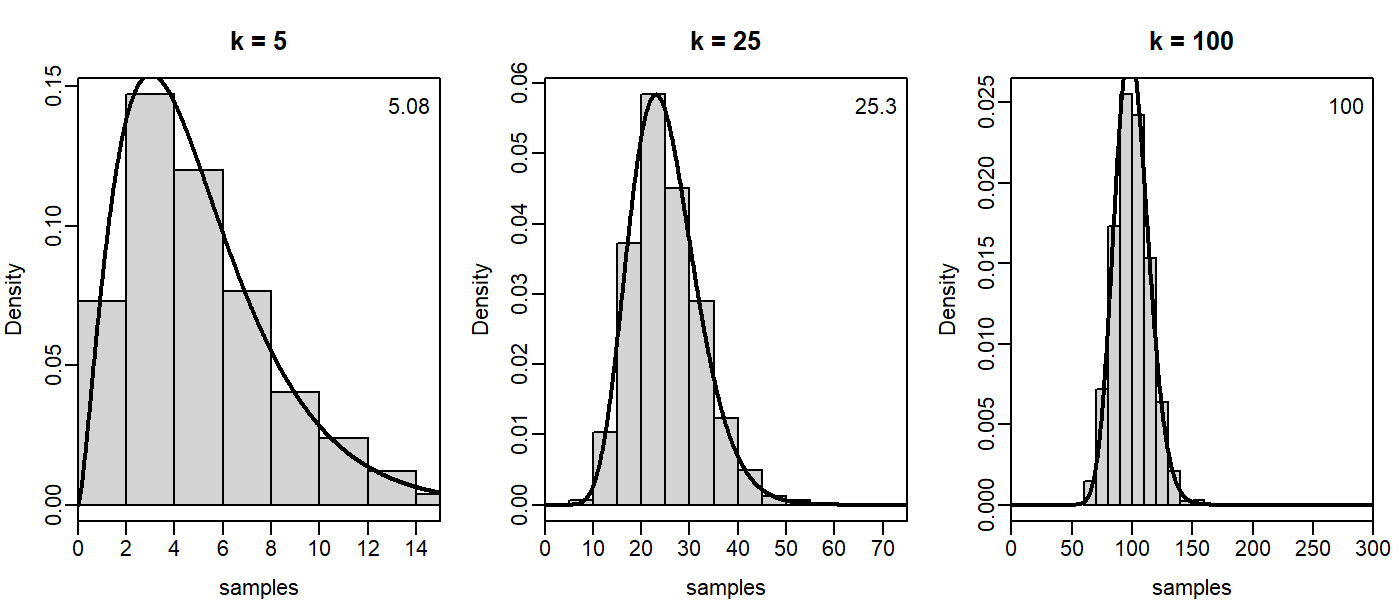
\includegraphics[width=5.5in]{Chap_2/Rejection_sampling_demo.png}
    \label{fig:Chap2_rejection}
\end{figure}

Comparing the Laplace approximation (Fig. \ref{fig:Chap2_laplace}) and Rejection Sampling (Fig. \ref{fig:Chap2_rejection}), we see that both approaches can be used to approximate the shape and resulting properties of a function.  However, the Laplace approximation is used in particular to approximate the area under a given curve (i.e., integrate a monotonic function), while sampling is typically used to calculate, e.g., the mean and standard deviation of a function when those are not already known.  We next demonstrate how these two approximations can be used for maximum likelihood estimation.  

\section{Estimating Heterogeneity using a Generalized Linear Mixed Model} \label{sec:Chap2_GLMM}

To summarize, recall that maximum likelihood involves identifying a vector of parameters that best explains the data:

\begin{equation}
    \hat{\theta} = \mathrm{argmax}_{\theta}( \log \mathcal{L}(\theta;y) )
\end{equation}
and we have now defined a marginal likelihood that involves integrating across random effects by approximating them as a normal distribution:

\begin{equation}
    \log \mathcal{L}(\theta;y) = \log \left( \int e^{f(\theta,\epsilon;y)} \mathrm{d}\epsilon \right)
\end{equation}
where \( f(\theta,\epsilon;y) = \log\left(\Pr(y|\theta,\epsilon) \Pr(\epsilon | \theta)\right) \) and this approximation in turn involves calculating \( \hat{\epsilon} \):

\begin{equation}
    \hat{\epsilon} = \mathrm{argmax}_{\epsilon} f(\theta,\epsilon;y) 
\end{equation}

So in terms of algorithm, using the Laplace approximation to fit a model with fixed and random effects involves:
\begin{enumerate}
    \item Defining the joint log-likelihood function \( f(\theta,\epsilon;y)\);

    \item Proposing a value of fixed effects \(\theta\);
    
    \item Optimize the joint log-likelihood with respect to random effects to identify \( \hat{\epsilon} \);
    
    \item Calculate the Hessian of \(f(\theta,\hat{\epsilon})\) with respect to \(\epsilon\) (termed the \myindex{inner Hessian matrix});
    
    \item Combine these two to approximate the log of the marginal likelihood;
    
\begin{equation} \label{eq:Chap2_laplace}
    \log \mathcal{L}(\theta;y) = f(\theta,\hat{\epsilon};y) - 0.5 \log(|\mathbf{H}|) + \frac{N}{2\log(2\pi)}
\end{equation}
    where \(N\) is the number of random effects, and noting that the term \(\frac{N}{2\log(2\pi)}\) does not depend upon parameters and can therefore be dropped without affecting the estimated parameters or standard errors;

    \item Propose a new value of fixed effects \(\theta\), repeat steps 3--5, compare the new and old log-marginal likelihoods, and accept whichever one is higher;
    
    \item Repeat step 6 until no further improvements are found;

    \item Calculate the Hessian of the log-marginal likelihood \(\log \mathcal{L}(\theta;y)\) with respect to fixed effects (termed the \myindex{outer Hessian matrix}).  The inverse of this outer Hessian matrix is then an estimate of the covariance in estimated fixed effects (recall Section \ref{sec:Chap1_likelihood_GLM}).
\end{enumerate}

To demonstrate this algorithm, we use real-world data measuring densities of different tree species in \myindex{Barro Colorado}, a long-term ecological experiment in Panama that records the exact location and species for every woody tree and shrub at least 1 cm in diameter within a 1 km by 500 m area over a sequence of years, 1982, 1985, 1990, 1995, 2000, 2005, and 2010  \cite{condit_dataset_2012}\footnote{We acknowledge R. Foster as plot founder and the first botanist able to identify so many trees in a diverse forest; R. Pérez and S. Aguilar for species identification; S. Lao for data management; S. Dolins for database design; plus hundreds of field workers for the census work, now over 2 million tree measurements; the National Science Foundation, Smithsonian Tropical Research Institute, and MacArthur Foundation for the bulk of the financial support. Data downloaded from \url{https://repository.si.edu/handle/10088/20925}.}.  This field experiment has yielded a wealth of insights about species turnover and community stability, and we here use it to illustrate that real-world data can be analyzed using these statistical principles.  We specifically illustrate data for \textit{Vismia baccifera} in 1985, and grid the data into 16 square cells each 250 m by 125 m (Fig. \ref{fig:Chap2_gridded}).

\begin{figure}[!ht]
    \caption[Gridded numerical abundance of \textit{Vismia baccifera} in Barro Colorado]{Gridded numerical abundance of \textit{Vismia baccifera} for 16 cells in the Barro Colorado census in 1985.}
    \centering
    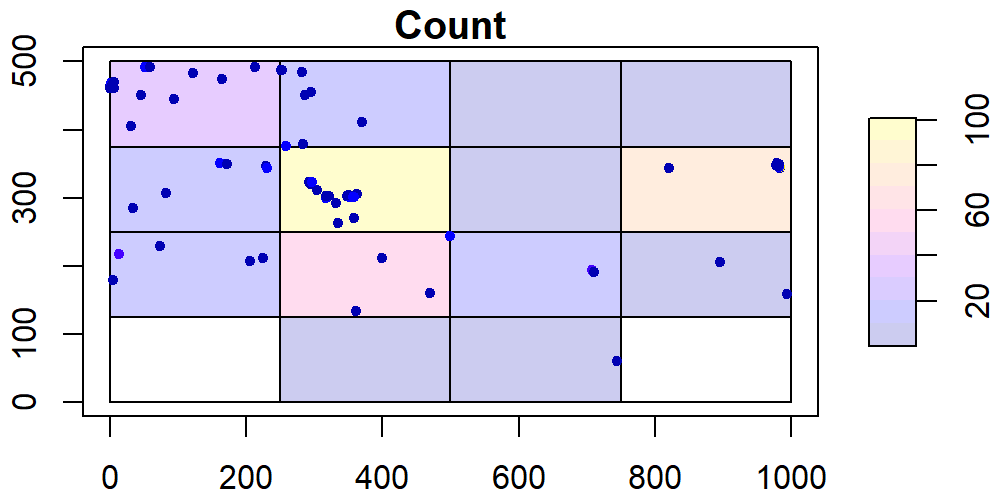
\includegraphics[width=4in]{Chap_2/gridded_density.png}
    \label{fig:Chap2_gridded}
\end{figure}

Given that we have counts in each grid cell, we might start by specifying a Poisson GLM. However, it is apparent that this would not capture the variation among sites.  Additionally, we might specifically wonder what is the variance of log-density among these sites.  To do this, we instead specify a generalized linear mixed model (GLMM).  

\begin{equation} \label{eq:Chap2_GLMM}
\begin{gathered}
    C_i \sim \mathrm{Poisson}( e^{\epsilon_i} ) \\ 
    \epsilon_i \sim \mathrm{Normal}( \mu, \sigma^2 ) 
\end{gathered}
\end{equation}
where \(\mu\) is the average log-density, \(\epsilon_i\) is the log-density for site \(i\), and \(\sigma^2\) is the variance in log-density among sites.  

\lstset{style=Rcode}
\lstinputlisting[language=R, label=code:Chap2-lme4-GLMM, firstline=33, lastline=35, caption=R code for fitting a log-linked Poisson distribution in a generalized linear mixed model using package \colorbox{backcolour}{lme4}., captionpos=t]{Chap_2/Demo_GLMM.R}

This model is easily fitted using many packages in R, and we use the \colorbox{backcolour}{lme4} package for simplicity \cite{bates_fitting_2015} (Code \ref{code:Chap2-lme4-GLMM}).  In this example, \colorbox{backcolour}{family $=$ poisson(link $=$ ``log")} specifies a log-linked linear predictor, and formula \colorbox{backcolour}{Count $\sim$ 1 + (1 $\vert$ Site)} indicates that we want to estimate the intercept (representing log-density \(\mu\)) as well as an additional intercept as random effect for each site (representing the centered deviation \(\epsilon_i-\mu\) for each \(i\)).  This function then generates a wide range of output, including the intercept and standard deviation estimates, as well as indicating that \colorbox{backcolour}{lme4} is already using the Laplace approximation:

%\verbatiminput{Chap_2/Lme_output.txt}
\lstset{style=Routput}
\lstinputlisting[language=R]{Chap_2/Lme_output.txt}

\lstset{style=Rcode}
\lstinputlisting[language=R, label=code:Chap2-joint-likelihood, firstline=44, lastline=60, caption=R code for joint likelihood of a log-linked Poisson GLMM., captionpos=t]{Chap_2/Demo_GLMM.R}

We again want to replicate this calculation using lower-level methods that can subsequently be extended.  To do so, we implement the inner and outer optimizers in R.  We first define a function that calculates the joint likelihood (Code \ref{code:Chap2-joint-likelihood}). We then use this to define a function that maximizes the joint likelihood with respect to random effects, calculates the inner Hessian matrix, and assembles the Laplace approximation to the marginal likelihood (Code \ref{code:Chap2-inner-optimizer}).  We later call this the \myindex{inner optimizer}.  Finally, we use an optimizer to identify the maximum likelihood estimates for fixed effects (Code \ref{code:Chap2-outer-optimizer}), which we later call the \myindex{outer optimizer}.  Inspecting estimates (Table \ref{tab:Chap2_R}) shows that they agree with those from \colorbox{backcolour}{lme4}.  

\lstset{style=Rcode}
\lstinputlisting[language=R, label=code:Chap2-inner-optimizer, firstline=64, lastline=75, caption=R code calculating the marginal likelihood by implementing an inner optimizer and calculating the Laplace approximation to the marginal likelihood., captionpos=t]{Chap_2/Demo_GLMM.R}

\lstset{style=Rcode}
\lstinputlisting[language=R, label=code:Chap2-outer-optimizer, firstline=79, lastline=98, caption=R code for maximizing the marginal likelihood using an outer optimizer., captionpos=t]{Chap_2/Demo_GLMM.R}

\begin{table}
  \catcode`"=9
  \centering
    \csvreader[
      tabular=|c|r|r|,
      table head=\hline \bfseries{} & \bfseries{Estimate} & \bfseries{Std. Error} \\\hline,
      late after last line=\\\hline % horizontal line at the end of the table
    ]{Chap_2/opt1_output.csv}{}{\csvlinetotablerow}
  \caption[Estimated parameters using Laplace approximation in R]{Estimated parameters and standard errors using the Laplace approximation implemented using custom code in R.}
  \label{tab:Chap2_R}
\end{table}

For illustration, we also extend this demonstration to include additional code that applies a finite-difference approximation to obtain the gradient of the marginal likelihood function with respect to fixed effects (see Table \ref{tab:Chap1_differentiation}).  We can then use this gradient to aid the process of identifying the maximum-likelihood estimates for fixed effects in the outer optimizer (Code \ref{code:Chap2-outer-optimizer-finite-difference}). Inspecting estimates now shows that estimates more closely agree with lme4 (comparing Tables \ref{tab:Chap2_TMB} and \ref{tab:Chap2_R_gradients}), and that the final gradient of the log-marginal likelihood is suitably low (as required for a maximum likelihood model to be converged).

\lstset{style=Rcode}
\lstinputlisting[language=R, label=code:Chap2-outer-optimizer-finite-difference, firstline=108, lastline=137, caption=R code for adding finite-difference gradient for outer optimizer using Laplace approximation for mixed-effect estimation., captionpos=t]{Chap_2/Demo_GLMM.R}

\begin{table}
  \caption[Estimated parameters using Laplace approximation in R using gradients]{Estimated parameters, standard errors, and final gradients using the Laplace approximation implemented using custom code in R that utilizes finite-difference gradients.}
  \catcode`"=9
  \centering
    \csvreader[
      tabular=|c|r|r|r|,
      table head=\hline \bfseries{} & \bfseries{Estimate} & \bfseries{Std. Error} & \bfseries{Final gradient} \\\hline,
      late after last line=\\\hline % horizontal line at the end of the table
    ]{Chap_2/opt2_output.csv}{}{\csvlinetotablerow}
  \label{tab:Chap2_R_gradients}
\end{table}

This process of writing an inner and outer optimizer and then the gradient function is cumbersome.  We therefore turn to TMB to automate the entire process, including calculating the gradients of the joint likelihood, computing the Hessian and Laplace approximation, and computing the gradient of that Laplace approximation to the log-marginal likelihood with respect to fixed effects.  As before, this involves writing the joint negative log-likelihood \( f(\theta, \epsilon | y) \) in a template file in C++ (Code \ref{code:Chap2-TMB-GLMM}).  This template file is then compiled and linked, and then the TMB object is built and optimized within R (Code \ref{code:Chap2-R-interface}).  By doing this, TMB automatically implements the inner optimizer while providing both the marginal log-likelihood and its gradients for use in an outer optimizer within R. Inspecting estimates, it agrees more closely with \colorbox{backcolour}{lme4} than either implementation using base R (while also being much faster to write and run).

\lstset{style=TMBcode} 
\lstinputlisting[language=c++, label=code:Chap2-TMB-GLMM, caption=TMB code for a log-linked Poisson generalized linear mixed model., captionpos=t]{Chap_2/poisson_glmm.cpp} 

\lstset{style=Rcode} 
\lstinputlisting[language=R, label=code:Chap2-R-interface, firstline=148, lastline=166, caption=R code for running the generalized linear mixed model implemented using TMB., captionpos=t]{Chap_2/Demo_GLMM.R}

\begin{table}
  \caption[Estimated parameters using Laplace approximation in TMB]{Estimated parameters, standard errors, and final gradients using the Laplace approximation implemented using TMB.}
  \catcode`"=9
  \centering
    \csvreader[
      tabular=|c|r|r|r|,
      table head=\hline \bfseries{} & \bfseries{Estimate} & \bfseries{Std. Error} & \bfseries{Final gradient} \\\hline,
      late after last line=\\\hline % horizontal line at the end of the table
    ]{Chap_2/tmb_glmm.csv}{}{\csvlinetotablerow}
  \label{tab:Chap2_TMB}
\end{table}

We also approximate the uncertainty in estimated fixed effects \( \mathbf{\theta} \) or predicted random effects \( \mathbf{\epsilon} \) by constructing the \myindex{joint precision matrix} \(\mathbf{Q}_{joint}\):

\begin{equation} \label{eq:Chap2_joint_precision}
    \mathbf Q_{joint} = 
    \begin{pmatrix}
      \mathbf H_1 & -\mathbf{H_1 G} \\
      -\mathbf{G^t H_1} & \mathbf{G^t H_1 G + H_2}
    \end{pmatrix}
\end{equation}
where \( \mathbf H_2 \) is outer Hessian matrix, \( \mathbf H_1 \) is the inner-Hessian matrix, and \( \mathbf G \) is the matrix of gradients of predicted random effects with respect to fixed effects (the \myindex{outer Jacobian matrix}).  This construction of \( \mathbf Q \) represents the precision (inverse-variance) arising from uncertainty about the value of fixed effects \(\mathbf H_1\), uncertainty about the random effects given estimated fixed effects \(\mathbf H_2\), how uncertainty about fixed effects affects uncertainty about random effects \( \mathbf{H_1 G} \), and uncertainty about random effects accumulated from fixed effects \(\mathbf{G^t H_2 G}\).  Inverting this joint precision then estimates the uncertainty in random effects \cite{kass_approximate_1989}.  We can calculate this using our custom version of the Laplace approximation (Code \ref{code:Chap2-R-joint-precision}), but TMB calculates it much faster automatically.    

\lstset{style=Rcode} 
\lstinputlisting[language=R, label=code:Chap2-R-joint-precision, firstline=176, lastline=190, caption=R code for calculating the joint precision matrix from the inner and outer Hessian matrices., captionpos=t]{Chap_2/Demo_GLMM.R}

Similar to Section \ref{sec:Chap2_Laplace}, we can also compare the Laplace approximation with a sample-based approximation.  In this case, we use \myindex{Markov Chain Monte Carlo} (MCMC) and specifically the No-U-Turn-Sampler NUTS \cite{hoffman_no-u-turn_2014} as implemented in Stan (see \cite{monnahan_faster_2017} for an accessible introduction to NUTS). MCMC generally involves generating a chain of samples from the \myindex{posterior distribution} (the product of the the joint likelihood function and Bayesian priors for fixed effects).  In this case, we do not explicitly specify any Bayesian priors, so implicitly we use an uniform and unbounded prior for all fixed effects.

Conveniently, users can run Stan algorithms on a TMB object using R-package \colorbox{backcolour}{tmbstan} \cite{monnahan_no-u-turn_2018} with no changes needed when defining the joint negative log-likelihood (Code \ref{code:Chap2-tmbstan}).  We compare these approaches for illustration purposes, and note that a real-world application would require consideration of Bayesian priors and post-hoc exploration of their impact on results.  We also note that NUTS could instead be run on the log-marginal likelihood (calculated using the Laplace approximation) or on the joint negative log-likelihood (as used during the inner optimization step).  Any difference between these two then indicates either error in the MCMC sampling algorithm or the Laplace approximation, and therefore any difference can be used to indicate that further investigation is needed.  We then compare the estimated densities obtained from both the Laplace approximation and NUTS sampling (Fig. \ref{fig:Chap2_predictions}), and see that these are indistinguishable by eye (despite NUTS including implicit uniform priors).


\lstset{style=Rcode}
\lstinputlisting[language=R, label=code:Chap2-tmbstan, firstline=240, lastline=241, caption=R code for running STAN to sample from the generalized linear mixed model implemented using TMB., captionpos=t]{Chap_2/Demo_GLMM.R}

\begin{figure}[!ht]
    \caption[Prediction of gridded abundance using Laplace approximation or STAN]{Predictions of gridded numerical abundance for 16 cells using the Laplace approximation or No-U-Turn-Sampling, both implemented using TMB and using the same color scale as Fig. \ref{fig:Chap2_gridded}.}
    \centering
    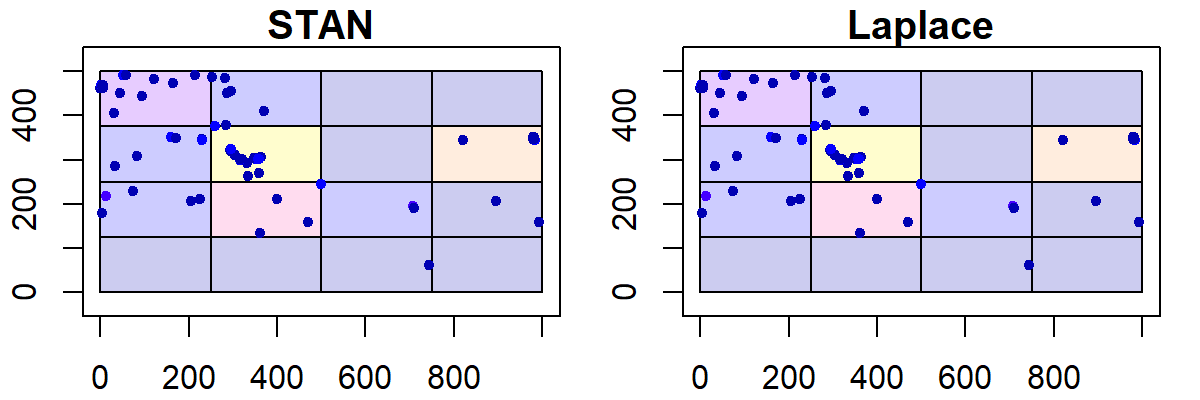
\includegraphics[width=5.5in]{Chap_2/gridded_predictions.png}
    \label{fig:Chap2_predictions}
\end{figure}

As noted in \ref{sec:Chap2_why}, hierarchical models are useful in part because they provide an objective way to implement \textit{shrinkage}.  To explain this in detail, we introduce the notation for a \myindex{generalized additive model} (GAM) \cite{wood_generalized_2006,hastie_generalized_1990}.  Similar to a GLM, a GAM identifies parameters by maximizing an objective function \(\mathcal{P}\).  It specifically calculates this objective function as the probability of the data given parameters but also includes an additional penalty on estimated coefficients:

\begin{equation}
    \log \mathcal{P}(\mathbf{\theta};Y) = \log \Pr(Y|\theta) - \lambda \mathbf{\theta^T S \theta} 
\end{equation}
where \(\mathbf{S}\) is a matrix that represents penalties on GAM coefficients.  Comparing this with maximum likelihood estimation (Eq. \ref{eq:Chap2_laplace}), we see that the GAM requires specifying a penalty matrix \(\mathbf{S}\) and identifying the penalty \(\lambda\), where the latter can be tuned based on fit to the data using a metric like \textit{generalized cross-validation}.  By contrast, maximum likelihood automatically estimates the penalty \(0.5\log(|\mathbf{H}|)\) during parameter estimation (Fig. \ref{fig:Chap2_shrinkage}). In GLMMs such as this, the penalty term \(0.5\log(|\mathbf{H}|)\) decreases as the variance of random effects increases, such that the marginal likelihood is maximized at a higher estimate of variance than the joint likelihood.  In fact, the joint likelihood typically increases infinitely as the variance of random effects approaches zero, and the log-determinant of the Hessian is needed to pull the maximum likelihood estimate away from this degenerate solution.  

Despite these differences between GLMMs and GAMs, both models include a component that \textit{shrinks} the coefficients towards zero.  Both are therefore ways of implementing a shrinkage estimator.  Shrinkage estimation can then bridge continuously between two different generalized linear models:
\begin{itemize}
    \item \textit{Intercept-only GLM}:  as the shrinkage becomes large (i.e., \(\sigma\) becomes small or \(\lambda\) becomes large), then \(\epsilon_i=\mu\) for all sites in the GLMM or GAM and these approach a GLM with only a single intercept;

    \item \textit{Site-level GLM}: as the shrinkage becomes large (i.e., variance \(\sigma^2\) becomes large or penalty \(\lambda\) becomes small), then \(\epsilon_i+\mu\) will approach the estimates that arise fitting a GLM with an intercept for each site.
\end{itemize}
The site-level GLM has more parameters (one intercept for each site) than the intercept-only GLM (one intercept for all sites).  Intuitively then, using a shinkage estimator (whether GLMM or GAM) to estimate parameters results in an \textit{effective degrees of freedom} that is intermediate between these two extremes. 

\begin{figure}[!ht]
    \caption[Illustrating shrinkage in a generalized linear mixed model]{Depiction of shrinkage in the generalized linear mixed model (see Fig. \ref{fig:Chap2_gridded}), showing (top panel) the joint log-likelihood, marginal log-likelihood, and the penalty term \(0.5\log(|\mathbf{H}|)\) calculated from the inner Hessian matrix \(\mathbf{H}\) (with maximum likelihood estimated shown as dotted vertical line), where the marginal loglikehood (black) is the joint loglikelihood (blue line) minus the penalty (red line) plus a constant. Also showing (bottom panel) the estimates of each site-level log-density for each site (y-axis) for different values of the random effect standard deviation (x-axis, using a log-scale), with the intercept-only GLM and site-level GLM estimates shown as green bullets.}
    \centering
    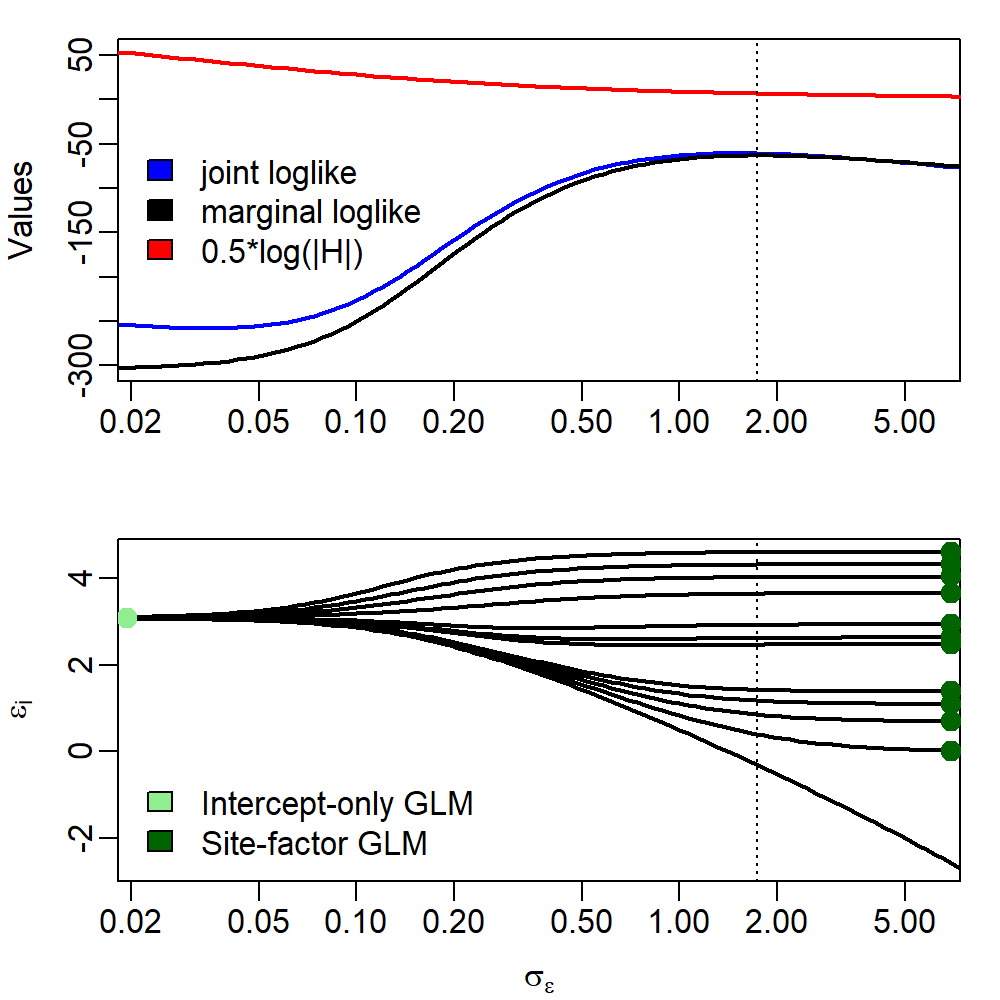
\includegraphics[width=5.5in]{Chap_2/Shrinkage.png}
    \label{fig:Chap2_shrinkage}
\end{figure}

We have illustrated that including random effects has many practical benefits (listed in Section \ref{sec:Chap2_why}).  However, they also complicate the evaluation of model fit and interpretation of residuals. To see this, recall from Section \ref{sec:Chap1_evaluating_model_fit} that we can calculate residuals by comparing model predictions \(\hat Y\) with observations \(Y\), and can use residuals to evaluate fit by constructing a quantile-quantile plot or applying a statistical test.  However, the mixed-effects model now has two apparent ways to calculate residuals:
\begin{itemize}
    \item \textit{Conditional residuals} involve calculating model predictions conditional on maximum likelihood estimates of fixed effects \(\hat \theta\) and empirical Bayes predictions of random effects \(\hat \epsilon\);

    \item \textit{Simulation residuals} involve acknowledging that random effects are estimated from a distribution \(\hat p(\epsilon) \propto \Pr(Y | \hat{\theta}, \mathbf{\epsilon}) \Pr( \mathbf{\epsilon} | \hat{\theta})\) (recall Eq. \ref{eq:Chap2_empirical_bayes}).  We could then simulate the value of random effects from this distribution, calculate model predictions given those simulated values, and then calculate residuals.  
\end{itemize}
From this description, it is perhaps apparent that conditional residuals are easier to compute but do not properly acknowledge that random effects are estimated from a distribution.  As a result, we cannot compute the expected distribution for model residuals under a properly specified model, and cannot use residuals to determine whether the model departs from this expectation.  However, simulation residuals also pose a subtle problem, because the predictive distribution \(\Pr(Y_i|\hat \theta, \hat p(\epsilon))\) for datum \(Y_i\) is informed by its observed value via the estimated distribution of random effects \(\hat p(\epsilon)\). Calculating residuals in this way is circular (i.e., residuals for each datum are calculated from a predicted distribution that is informed by that datum) and this circularity then results in residuals that are not statistically independent.  This lack of independence again makes it difficult to compute a ``null distribution" for model residuals, or interpret whether any patterns are a substantial departure from this.  

To address these projects arising from conditional and simulated residuals, TMB includes a generic implementation for \textit{one-step-ahead} (``OSA") residuals \cite{thygesen_validation_2017}.  Calculating OSA residuals involves ordering the data and constructing the predictive distribution for each datum conditional only on preceding data.  These OSA residuals are then statistically independent, and simulations confirm that OSA residuals have better performance for identifying model mis-specification than either conditional or marginal residuals \cite{trijoulet_performance_2020}.    

\section{Inner Hessian Sparsity and Conditional Independence} \label{sec:Chap2_Hessian_sparsity}

We have seen that we can implement the Laplace approximation both in custom R code, and via TMB, and that this approximation gives very similar estimates of density to a sampling-based approximation or high-level functions in R.  We next discuss the computational aspects of the Laplace approximation in more detail.

In our example, we have 16 coefficients in random effect \(\epsilon\), such that the \myindex{inner Hessian matrix} is 16 x 16. The Laplace approximation involves calculating the log-determinant of this inner Hessian matrix (Eq. \ref{eq:Chap2_laplace}), which becomes more computationally expensive as the number of random effects increases. To compensate, TMB tracks the inner Hessian as a \myindex{sparse matrix} using a triplet format, i.e., where it records the row index, column index, and value of the inner hessian matrix only for a pair of random effects that are correlated conditional upon a fixed value of parameters.  This inner Hessian is a diagonal matrix in our example (i.e., the second derivative of any two sites is zero) and is therefore as sparse as possible for the GLMM we are using.  We will often want to plot this inner Hessian to check its sparsity pattern (Fig. \ref{fig:Chap2_hessian}), where this image shows a nonzero value on the diagonal and is exactly zero along the off-diagonal.

\begin{figure}[!ht]
    \caption[Sparsity pattern for generalized linear mixed model]{Hessian matrix for the 16 values of \(\epsilon\) in our GLMM example, where white cells are known to be exactly zero and hence not tracked in the sparse representation of the matrix.}
    \centering
    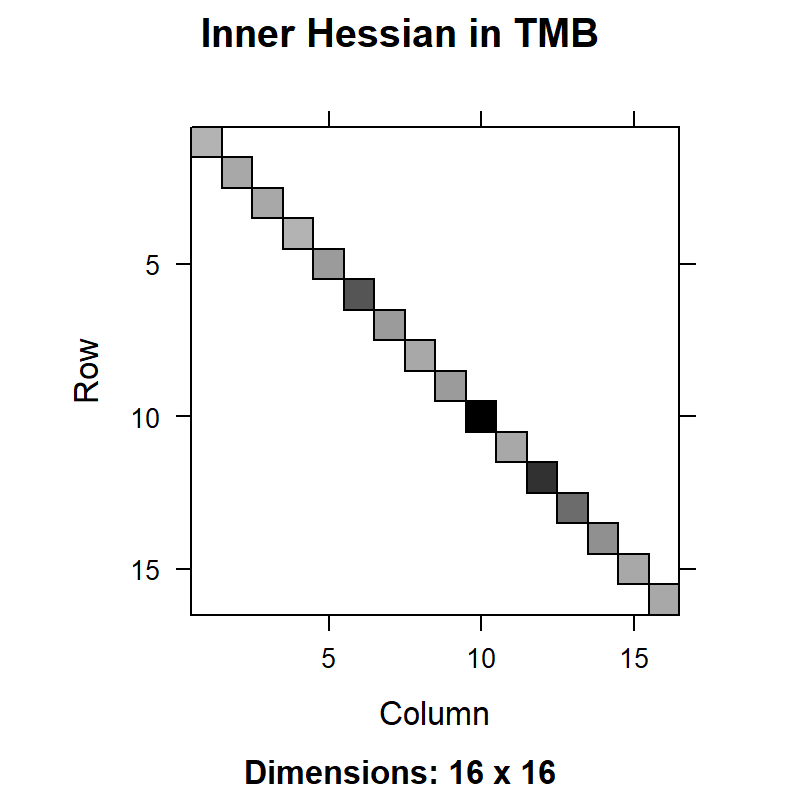
\includegraphics[width=4in]{Chap_2/TMB_hessian.png}
    \label{fig:Chap2_hessian}
\end{figure}

There are several ways to conceptualize the sparsity of the inner Hessian:
\begin{enumerate}
    \item \textit{Conditional independence}\index{conditional independence}:  if a random effect \(\epsilon_1\) is independent of another \(\epsilon_2\) conditional upon a fixed value of for other fixed and random effects, then the inner Hessian matrix will be zero for that pair of random effects.  

    \item \textit{Separability}\index{separability}:  se have seen that the marginal likelihood is calculated by computing a multidimensional integral across random effects:

\begin{equation}
    \mathcal{L}( \theta; y ) = \int \Pr(y | \theta, \epsilon) \Pr( \epsilon | \theta) \text{d}\epsilon  
\end{equation}
    
    However, this multidimensional integral can in some times be replaced by a series of lower-dimensional integrals.  For example, in our GLMM example, we can replace a 16-dimensional integral with 16 1-dimensional integrals.
    
\begin{equation}
    \mathcal{L}( \theta; y ) = \prod_{i=1}^{n_i} \int \Pr(Y_i | \theta, \epsilon_i) \Pr( \epsilon_i | \theta) \text{d}\epsilon_i 
\end{equation}
    
    In other cases, the integral can be broken into multiple blocks. When using the Laplace approximation, breaking the integral into blocks is identical to specifying that the inner Hessian matrix has that same block structure. 
    
    \item \textit{Graphical blocking}\index{graphical blocking}:  a statistical model can generally be written as a graph where fixed effects, random effects, and data are vertices and any probability distribution that involves any pair of parameters is represented by an edge (Fig. \ref{fig:Chap2_graph}).  In a graphical model, two random effects will be correlated if either (1) they both point at a single datum, or (2) they have an arrow pointing from one to the other.  In this case, however, there are no arrows between random effects (diamond), and similarly, there are no data that are connected by multiple random effects.  Therefore, each random effect is independent conditional upon the value of fixed effects.  
    
\begin{figure}[!ht]
    \caption[Graphical illustration of GLMM parameters and data]{A graphical model for three of the 16 sites in our GLMM example (Eq. \ref{eq:Chap2_GLMM}), showing data as boxes, random effects as diamonds, and fixed effects as circles, and showing the conditional dependencies as arrows.}
    \centering
    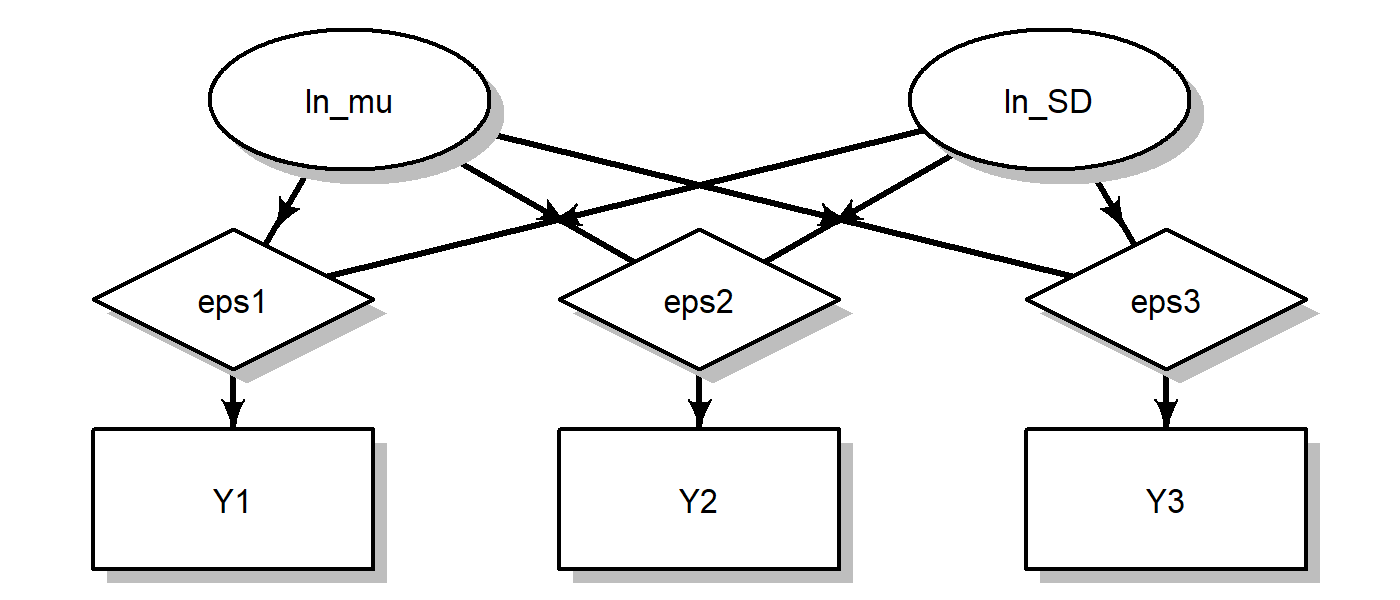
\includegraphics[width=5.5in]{Chap_2/graph.png}
    \label{fig:Chap2_graph}
\end{figure}

\end{enumerate}
Clearly, we are using similar terms across these three explanations, so stating them as separate interpretations is somewhat artificial.  However, each might be a convenient approach to think about sparsity in some cases.  These same principles apply in later models, where the inner Hessian has a more complicated structure.  Finally, we note that different parameterizations can result in an identical maximum likelihood estimate but different sparsity, and typically the more sparse version will run faster and with less computer memory required.  

We also emphasize that the Laplace approximation involves alternating between an inner and an outer optimizer (see Code \ref{code:Chap2-inner-optimizer} and \ref{code:Chap2-outer-optimizer}). This process will converge very slowly on the maximum likelihood estimate whenever fixed and random effect estimates are highly correlated (i.e., the Hessian of the joint likelihood has higher values between fixed and random effects).  For example, our GLMM could instead have been written as:

\begin{equation} \label{eq:Chap2_slow_laplace}
\begin{gathered}
    C_i \sim\ \mathrm{Poisson}( e^{\mu+\epsilon_i} ) \\ 
    \epsilon_i \sim\ \mathrm{Normal}( 0, \sigma^2 )
\end{gathered}
\end{equation}
and this would result in identical estimates of fixed effects. However, it would also cause fixed effect \(\mu\) and random effect \(\epsilon\) to be highly correlated.  We encourage readers to change the R code to use this parameterization and see how it affects estimation performance in particular when not using gradient information.  

\section{Addressing Common Problems During Inner or Outer Optimization} \label{sec:Chap2_convergence_problems}

Finally, every analyst using TMB will encounter bugs and errors with some frequency:
\begin{itemize}
    \item \myindex{TMB syntax errors}:  some of these are evident when running the \colorbox{backcolour}{compile} function to compile a CPP script using TMB and the file fails to compile.  Typically, some informative (although difficult to read) messages are displayed in the terminal that can give clues to where the syntax error arises;

    \item \textit{Out-of-bounds errors}\index{out-of-bounds errors}:  other bugs occur when running the \colorbox{backcolour}{MakeADFun} function to build a TMB object.  These typically occur when the CPP code is attempting to access a vector, matrix, or array value that is ``out of bounds".  This occurs, e.g., when defining a vector of length 10 but trying to access the 11th element.  This type of error may crash the R session.
\end{itemize}
These compiler and out-of-bounds errors are programming bugs, and addressing them in detail is  outside the scope of this book.  However, we do specifically note two more types of error that have a statistical interpretation, where explaining their cause and potential solution can provide insight into model structure.  These errors occur either in the outer or inner optimizer, and we further address them in detail below.

\subsection{Inner Hessian failure}

The first type of error occurs during the inner optimizer, where users might see a message like below:

%\verbatiminput{Chap_2/Inner_hessian_error.txt}
\lstset{style=Routput}
\lstinputlisting[language=R]{Chap_2/Inner_hessian_error.txt}
where the final line is the terminal error message.  For demonstration purposes, we have intentionally caused this error to occur by specifying an additional random effect that has no effect on the joint likelihood, i.e., by specifying \colorbox{backcolour}{params\$eps\_i = rep(0, nrow(Data)+1)}, such that the final element of vector \colorbox{backcolour}{eps\_i} is not used in the calculation of either the probability of random effects or the likelihood of data.  The terminal message indicates that the maximum gradient component (``mgc") of the inner optimizer has become close to zero (abbreviated in the R-terminal messages as \colorbox{backcolour}{mgc: 1.350213e-08}).  At this point, the inner optimizer stops because the low gradient suggests that the inner optimizer is converged.  TMB then calculates the Hessian matrix, and attempts to calculate its determinant for use in the Laplace approximation (Eq. \ref{eq:Chap2_laplace}).  However, the final element of \colorbox{backcolour}{eps\_i} has no effect on the joint likelihood, such that the gradient of the joint likelihood with respect to its value is zero.  Similarly, the matrix of second derivatives is zero for any row or column involving this value.  This then causes the Hessian matrix to not be invertible;  technically it is only positive semi-definite, and has an eigenvalue that is identical to zero, which when inverted would involve dividing by zero (see Section \ref{sec:Appendix_eigendecomposition}).  

\begin{figure}[!ht]
   \caption[Sparsity pattern for non-invertible inner Hessian matrix]{Hessian matrix for the 17 values of \(\epsilon\) in our GLMM example when intentionally including a random effect that has no effect on the joint likelihood and therefore causes an error when calculating the inner Hessian used in the Laplace approximation.}
    \centering
    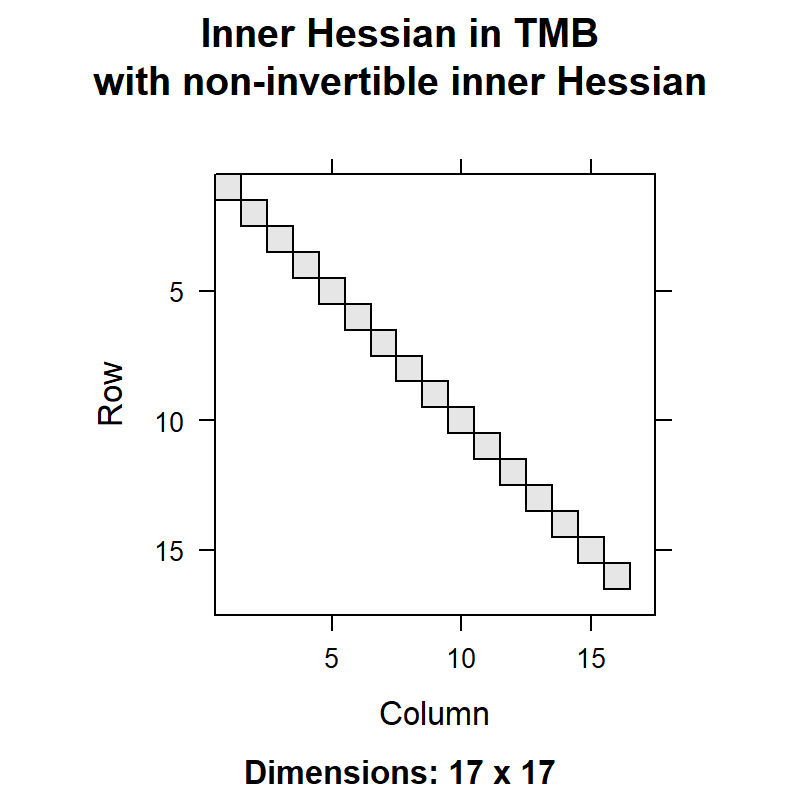
\includegraphics[width=4in]{Chap_2/TMB_hessian_bug.png}
     \label{fig:Chap2_TMB_hessian_bug}
\end{figure}

In this case, the error can be detected by extracting the inner Hessian using \colorbox{backcolour}{Obj\$env\$spHess(random=TRUE)}.  Plotting this immediately shows that the final random effect has no rows or columns that are non-zero (Fig. \ref{fig:Chap2_TMB_hessian_bug}).  In more complicated cases, we can instead build the model with all fixed effects ``mapped off", and instead optimize the joint log-likelihood with respect to random effects (Code \ref{code:Chap2-manual-inner-optimizer}).  This allows us to explore in detail what is happening during the inner optimizer, which is otherwise hidden from the user. This approach is helpful when the inner Hessian fails to converge for some values of fixed effects and not others.  

\lstset{style=Rcode}
\lstinputlisting[language=R, label=code:Chap2-manual-inner-optimizer, firstline=316, lastline=322, caption=R code for manually running the inner optimizer to diagnose lack-of-convergence., captionpos=t]{Chap_2/Demo_GLMM.R}

In more complicated cases, it might not be apparent what combination of random effects is causing the inner Hessian to not be invertible.  In this case, the analyst can extract the inner Hessian, calculate its eigendecomposition, and identify those eigenvalues that are zero (or very close to zero) (see Section \ref{sec:Appendix_eigendecomposition}).  The corresponding eigenvectors can then be inspected, to find what parameters are associated with non-invertible dimensions (Code \ref{code:Chap2-eigen-for-inner-hessian}).  This approach can then identify a linear combination of parameters that is not invertible, and can prompt further thought about model restrictions.  

\lstset{style=Rcode}
\lstinputlisting[language=R, label=code:Chap2-eigen-for-inner-hessian, firstline=326, lastline=331, caption=R code for identifying non-invertible axes of the inner Hessian matrix., captionpos=t]{Chap_2/Demo_GLMM.R}

\subsection{Outer Hessian failure} \label{sec:Chap2_outer_hessian_failure}

The second type of error occurs during the outer optimizer, where users might run \colorbox{backcolour}{sdreport} and then see that standard errors are missing:

%\verbatiminput{Chap_2/sdreport_error.txt}
\lstset{style=Routput}
\lstinputlisting[language=R]{Chap_2/sdreport_error.txt}
As indicated by the output, the Hessian of the outer optimizer (which optimizes fixed effects) is not positive definite.  We can again use \colorbox{backcolour}{optimHess} to construct and visualize the outer Hessian matrix, and inspect the eigendecomposition to determine which combination of parameters is responsible. 

Addressing these topics from a more theoretical perspective, we note that a model is \myindex{estimable} if and only if:
\begin{enumerate}
    \item we can identify a set of fixed effects that minimizes the negative marginal log-likelihood; and 

    \item the Hessian matrix is also positive definite.
\end{enumerate}
Therefore, optimizing and confirming that the outer Hessian is positive definite is sufficient to confirm that the model is estimable for given a particular data set \cite{hunter_rank_2009}.  Alternatively, a model may not be \myindex{identifiable}.  Identifiability refers to whether a model has parameters that could ever be estimable, given some ideal combination of data.  If the model is not identifiability then it can never be estimable for any data set \cite{jacquez_numerical_1985}.  From the law of contraposition, we can also see that, if a model is estimable for any single data set, then the model is identifiable.  On a practical level, it is often possible to specify a non-identifiable model in TMB;  in fact, that is what we did by intentionally introducing a fixed effect that had no role in calculating the joint likelihood.  In this case, we showed that we could detect that the model was not estimable for a simulated data set.  Alternatively, we fitted the log-linked Poisson GLMM in Section \ref{sec:Chap2_GLMM} and calculated its standard errors.  By observing that the model was estimable using that single data set, we also confirmed that the log-linked Poisson GLMM was identifiable. 

\section{Chapter Summary}

In summary we have showed that:
\begin{enumerate}
    \item Many real-world circumstances will result in a likelihood that cannot be easily written, either because model residuals are correlated and/or ecological processes involve unobserved (``latent") variables.  In these cases, it is helpful to formulate the model while including latent variables, and then obtain the likelihood by marginalizing across these variables.  This results in a marginal likelihood that can be optimized to identify maximum likelihood estimators for parameters;  
    
    \item The marginal likelihood can be used to identify maximum-likelihood estimates for variance parameters. The estimated variance then controls the magnitude of ``shrinkage," wherein random effects are pulled towards some specified average value.  This performs a similar role to the penalty term in a generalized additive model, and both provide a continuous bridge between two extremes along a continuum: either fitting a model without random effects, or fitting a model that treats each random effect as if it were estimated separately as a fixed effect;

    \item Marginalizing across latent variables requires a multidimensional integral if random effects are continuous, or summation if random effects are discrete-valued. The Laplace approximation is a convenient approximation to identify the area under a smooth function, and therefore can be used to integrate across random effects.  The Laplace approximation involves approximating a smooth function as if it where actually a multivariate normal distribution with the same peak and curvature.  This approximation requires identifying  the value of random effects that maximizes the joint likelihood, and then calculating the curvature of the joint likelihood around those values.   
    
    \item Using the Laplace approximation to fit a likelihood model with fixed and random effects involves an inner optimizer, which optimizes random effects conditional upon fixed effects and then calculates the Laplace approximation to the marginal likelihood. This inner optimizer is then embedded in an outer optimizer, which optimizes the fixed effects using the marginal likelihood.

    \item The work of coding the inner and outer optimizer can be automated using Template Model Builder, and the performance of the Laplace approximation can be explored by comparison with sample-based methods like MCMC or Rejection Sampling.  Errors arising during the inner or outer optimizers can often be diagnosed by extracting the inner or outer Hessian matrix, respectively, and then either visualizing this (in simple cases) or inspecting the eigendecomposition (in more complicated cases);

    \item The Laplace approximation is computationally efficient when the Hessian matrix used in the inner optimizer (called the ``inner Hessian") is sparse (i.e., contains many zeros).  Sparseness can be automatically detected and plotted, but can also be explored by thinking about conditional independence, writing out a separable integral for random effects, or constructing a graph of fixed effects, random effects, and data, and exploring how these are linked by components of the joint likelihood.
\end{enumerate}

\section{Exercises}


\begin{enumerate}
    \item \textit{Heterogeneity in proportions}:  we introduced the concept of compound distributions in Section \ref{sec:Chap2_compound_distribution}, and here expand this concept to represent heterogeneity in proportions.  To do so, imagine a survival experiment including 10 microcosms, each containing 20 individuals that are subject to some experimental treatment.  Imagine that some fraction \(p=0.5\) is expected to survive over the course of the experiment, such that the number of survivors \( C_i\) in each microcosm \(i\) is drawn from a Binomial distribution \( C_i \sim \mathrm{Binomial}(N=20,p=p_i)\) and where \(p_i = 0.5\) for each microcosm.  First, simulate data from one replicate of this experiment.  Then, fit a logit-linked generalized linear model using a Binomial distribution for survival in each microcosm (see Appendix \ref{sec:Appendix_links_and_distributions} for details), confirming identical results when using \colorbox{backcolour}{glm} or when coding the generalized linear model in TMB by modifying Code \ref{code:Chap1-TMB-GLM}.  Next, repeat the experiment, but simulating data where each microcosm has a different survival rate drawn from a uniform distribution, \( p_i \sim \mathrm{Uniform}(0.2,0.8) \) using \colorbox{backcolour}{p = runif(n=20,min=0.2,max=0.8)}.  How might you represent this heterogeneity in survival proportions within a generalized linear mixed model?  Consider modifying Code \ref{code:Chap2-TMB-GLMM} to represent microcosm-specific survival rates using a Beta distribution (i.e., calculating \colorbox{backblue}{jnll -= dbeta(p\_i,alpha,beta,true)} for the distribution of survival rates in each microcosm) while estimating two parameters \colorbox{backblue}{alpha} and \colorbox{backblue}{beta}, where the mean of the Beta distribution is then \(\frac{\alpha}{\alpha+\beta}\).  Please confirm that the estimated mean matches the true mean \( \E(p_i) = 0.5\) of the simulated Uniform distribution. 

    \item \textit{Comparison of residual estimators}:  in Section \ref{sec:Chap2_GLMM}, we fit a log-linked Poisson GLMM for gridded plant densities, and also introduce the distinction between conditional, marginal, and OSA residuals.  Please compute conditional, marginal and OSA residuals for that data set.  To do so, first review Section \ref{sec:Chap1_evaluating_model_fit} to calculate conditional residuals, i.e., by computing PIT residuals conditional on empirical Bayes predictions of random effects. Then consider calculating marginal residuals by using \colorbox{backcolour}{tmbstan} to sample from a single vector of random effects conditional on the maximum likelihood estimate of fixed effects, and computing PIT residuals for that vector of random effects.  Finally, modify Code \ref{code:Chap2-TMB-GLMM} to compute OSA residuals, consulting \colorbox{backcolour}{?oneStepPredict} to identify syntax for code changes and using \colorbox{backcolour}{method=``cdf"} to apply \colorbox{backcolour}{oneStepPredict} to these the discrete-valued data.  Next, simulate new data sets from the fitted model (i.e., new random effects conditional on estimated fixed effects, and data conditional on both), refit the model, and recompute these residuals.  How do the residuals using real-world data compare with residuals computed from a correctly specified model, and what does this suggest about inference from that original model?   
\end{enumerate}
 
     


